	\documentclass[12pt]{article}
	\title{\textbf{By the Rules: The Effect of Primary Rules on Turnout}}
	\author{Abe Winterscheidt}
	\usepackage{listings}
	\usepackage[export]{adjustbox}
	\lstdefinestyle{mystyle}{
		breaklines=true		
	}
	\lstset{style=mystyle}
	\usepackage{amssymb}
	\usepackage[margin=1in]{geometry}
	\usepackage{rotating}
	\usepackage{setspace}
	\usepackage{graphicx}
	\usepackage{float}
	\usepackage{booktabs} % For \toprule, \midrule and \bottomrule
	\usepackage{siunitx} % Formats the units and values
	\usepackage{pgfplotstable} % Generates table from .csv
	\usepackage{hanging}
	
\begin{document}
	\maketitle
	\begin{doublespace}
	\section{Introduction}
	The presidential primary elections held in the spring of each election cycle are essential to determining the country’s executive future. Democrats and Republicans pit their candidates against one another in a fight for the party’s delegates. Despite their importance in the electoral process, primaries see notoriously low turnout rates (Gans 2010). Turnout may be low due to a lack of campaign consistency as candidates take extended stays in states early in the cycle, but visit later states only briefly (Frederick 2012; McDonald \& Merivaki 2015). The lack of party resources in primaries limits candidates’ campaigning ability, and voters may see little benefit in staying informed about primary candidates (McDonald \& Merivaki 2015; Gerber et al. 2017). Incumbent years see fewer candidates in the incumbent party’s primaries – in most cases, only the incumbent themself runs.
\par
	Another factor that may impact primary turnout are primary rules. Generally, primaries fall into one of three categories: open, closed, or mixed. Geer (1986) defines these three primary types: open primaries are ones in which any registered voter may participate in a party’s primary regardless of their party affiliation, closed primaries limit participation to registered party members, and mixed primaries (or as Greer calls them “semi-closed” (1017)) are ones that are limited to registered party members but also allow independent voters to participate. There have been mixed results in tests of the effects of primary rules on turnout. Earlier studies find that closed primaries lead to higher levels of turnout (Norrander \& Smith 1985; Ranney 1977). More recent studies find evidence of the opposite: open primaries having higher turnout over closed primaries (Kaufmann, Gimpel, \& Hoffman 2003; Patterson 2009; Jewitt 2014; Hersh \& Ghitza 2018). Others still find no significant difference for between different eligibility rules (McDonald \& Merivaki 2015; Oliver 1996). Little, however, has been said about the specific role of mixed primaries. Kaufmann, Gimpel, \& Hoffman (2003) incorporate a dummy for mixed primaries but find no significant results compared to closed elections.
\par
	By comparing presidential primaries since 2000, I seek to find more recent trends in turnout in all three types of elections. I expect to find that open primaries see higher levels of turnout compared to both closed and mixed primaries, and that mixed primaries have higher levels of turnout than closed primaries. This relationship would be explained by the role of independent voters and dissenting counter-partisans in a party’s open (or mixed) elections. In particular, dissenting-counter partisans, those members of the other party who are dissatisfied with their party’s candidates, particularly in incumbent years, would increase the turnout in states with open primaries. I also expect to find that incumbent years see lower levels of turnout overall. 
	\section{Methodology}
	I will utilize two primary methods to examine the effect of primary rules on turnout. First, I conduct a series of comparison of mean t-tests between each of the three types of rules (open, closed, and mixed). Next, I will utilize a series of time-fixed-effects regressions to determine if a significant causal relationship exists between rule type and turnout.\par
	\subsection*{Data}
	Turnout and rule data were collected on both parties' primary elections in all five presidential cycles between 2000 and 2016 for fifty states and Washington, D.C. States in which Republicans and Democrats had different primary rules or had caucuses were omitted, leaving 141 of 255 possible data points. The 2004 and 2012 incumbent years saw the least consistency between parties' rules, possibly fueled by changes made by the incumbent party's such as cancelled primary elections, a testament to why voters may feel unimportant in the nominating process. The variable \textit{Type} was a categorical variable where open primaries are denoted with a value of 1, closed primaries are denoted with a value of 2, and mixed primaries are denoted with values of 3. \textit{Turnout} was measured as a percentage of the voting eligible population, which excludes felons and noncitizens who may otherwise be able to vote.
	\par
	\textit{Figure 1} shows a histogram of turnout in the dataset. While the distribution of the data is slightly right-skewed, the logarithm of turnout is far more left-skewed than the raw data is right-skewed. 
	\begin{figure}[H]
		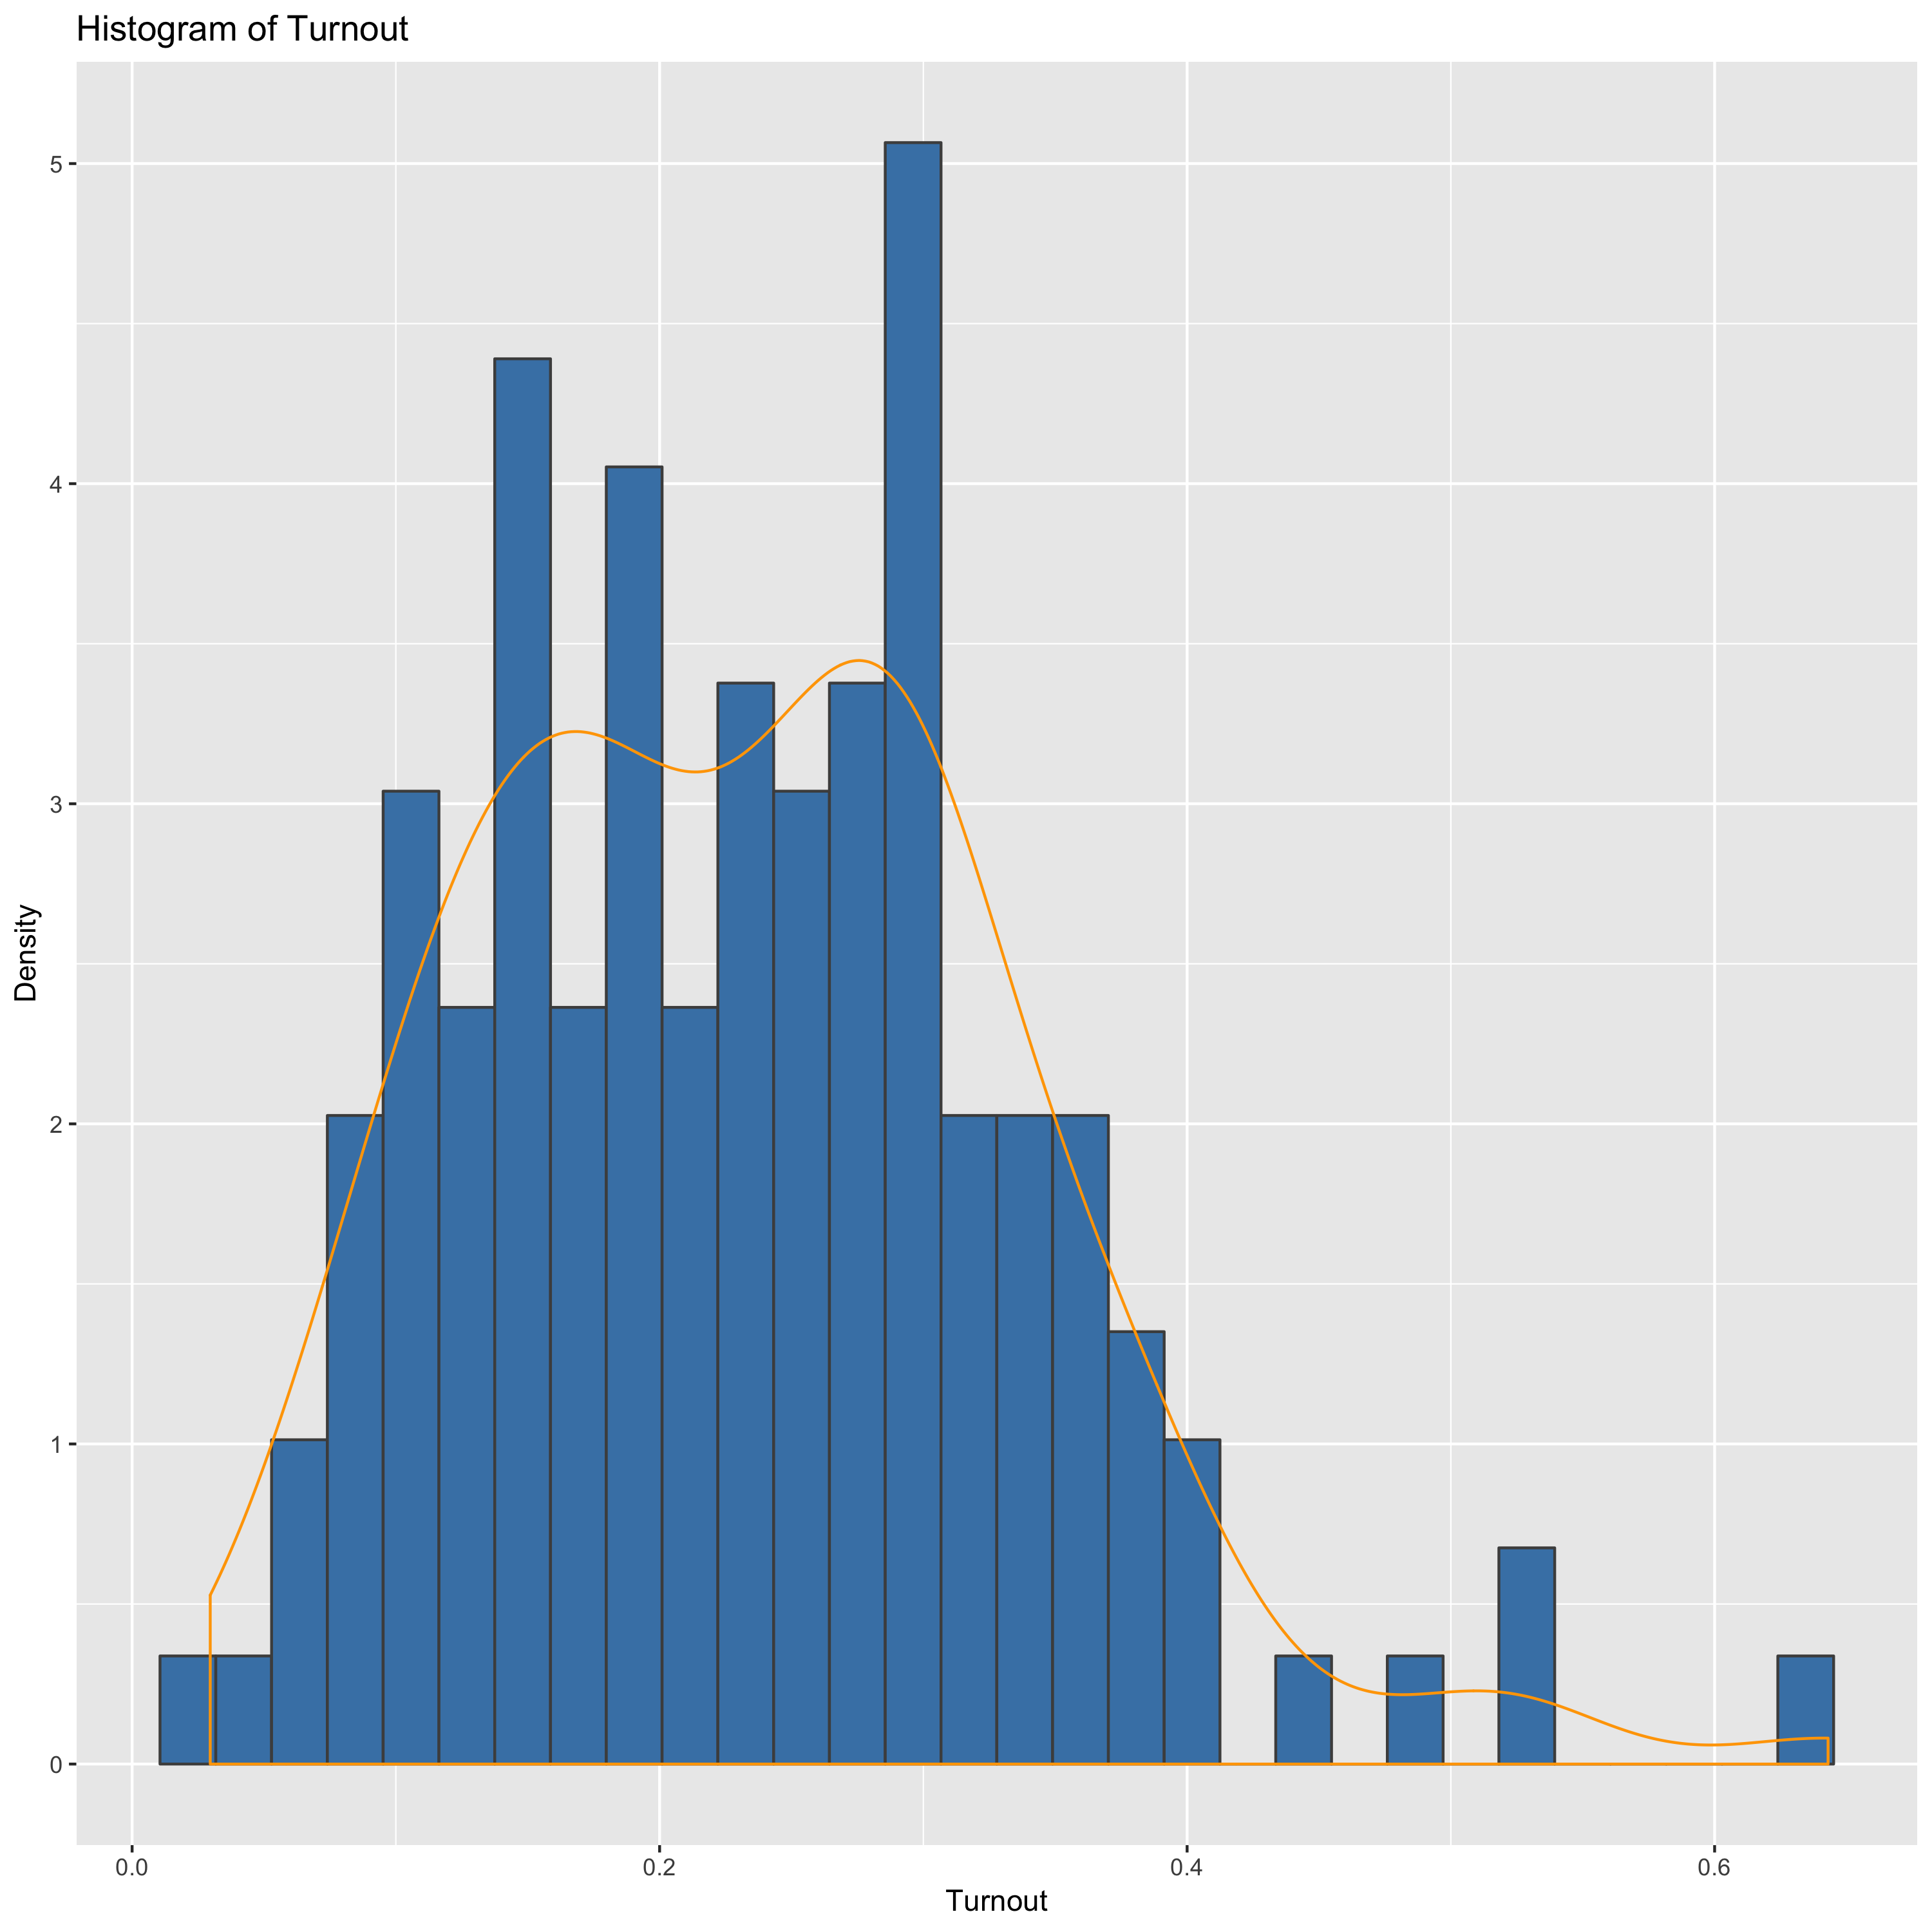
\includegraphics[width=0.3\textwidth, center]{H}
		\caption{Histogram of Primary Turnout}
		\label{fig:figure1}
	\end{figure}
	Similar distributions are seen in \textit{Figure 2}, where turnout is split up by primary types. Of the three types of rules, mixed primaries had the most normal distribution. Once again, the distributions of the logarithm of turnout split by type was skewed far to the left.
	\begin{figure}[H]
		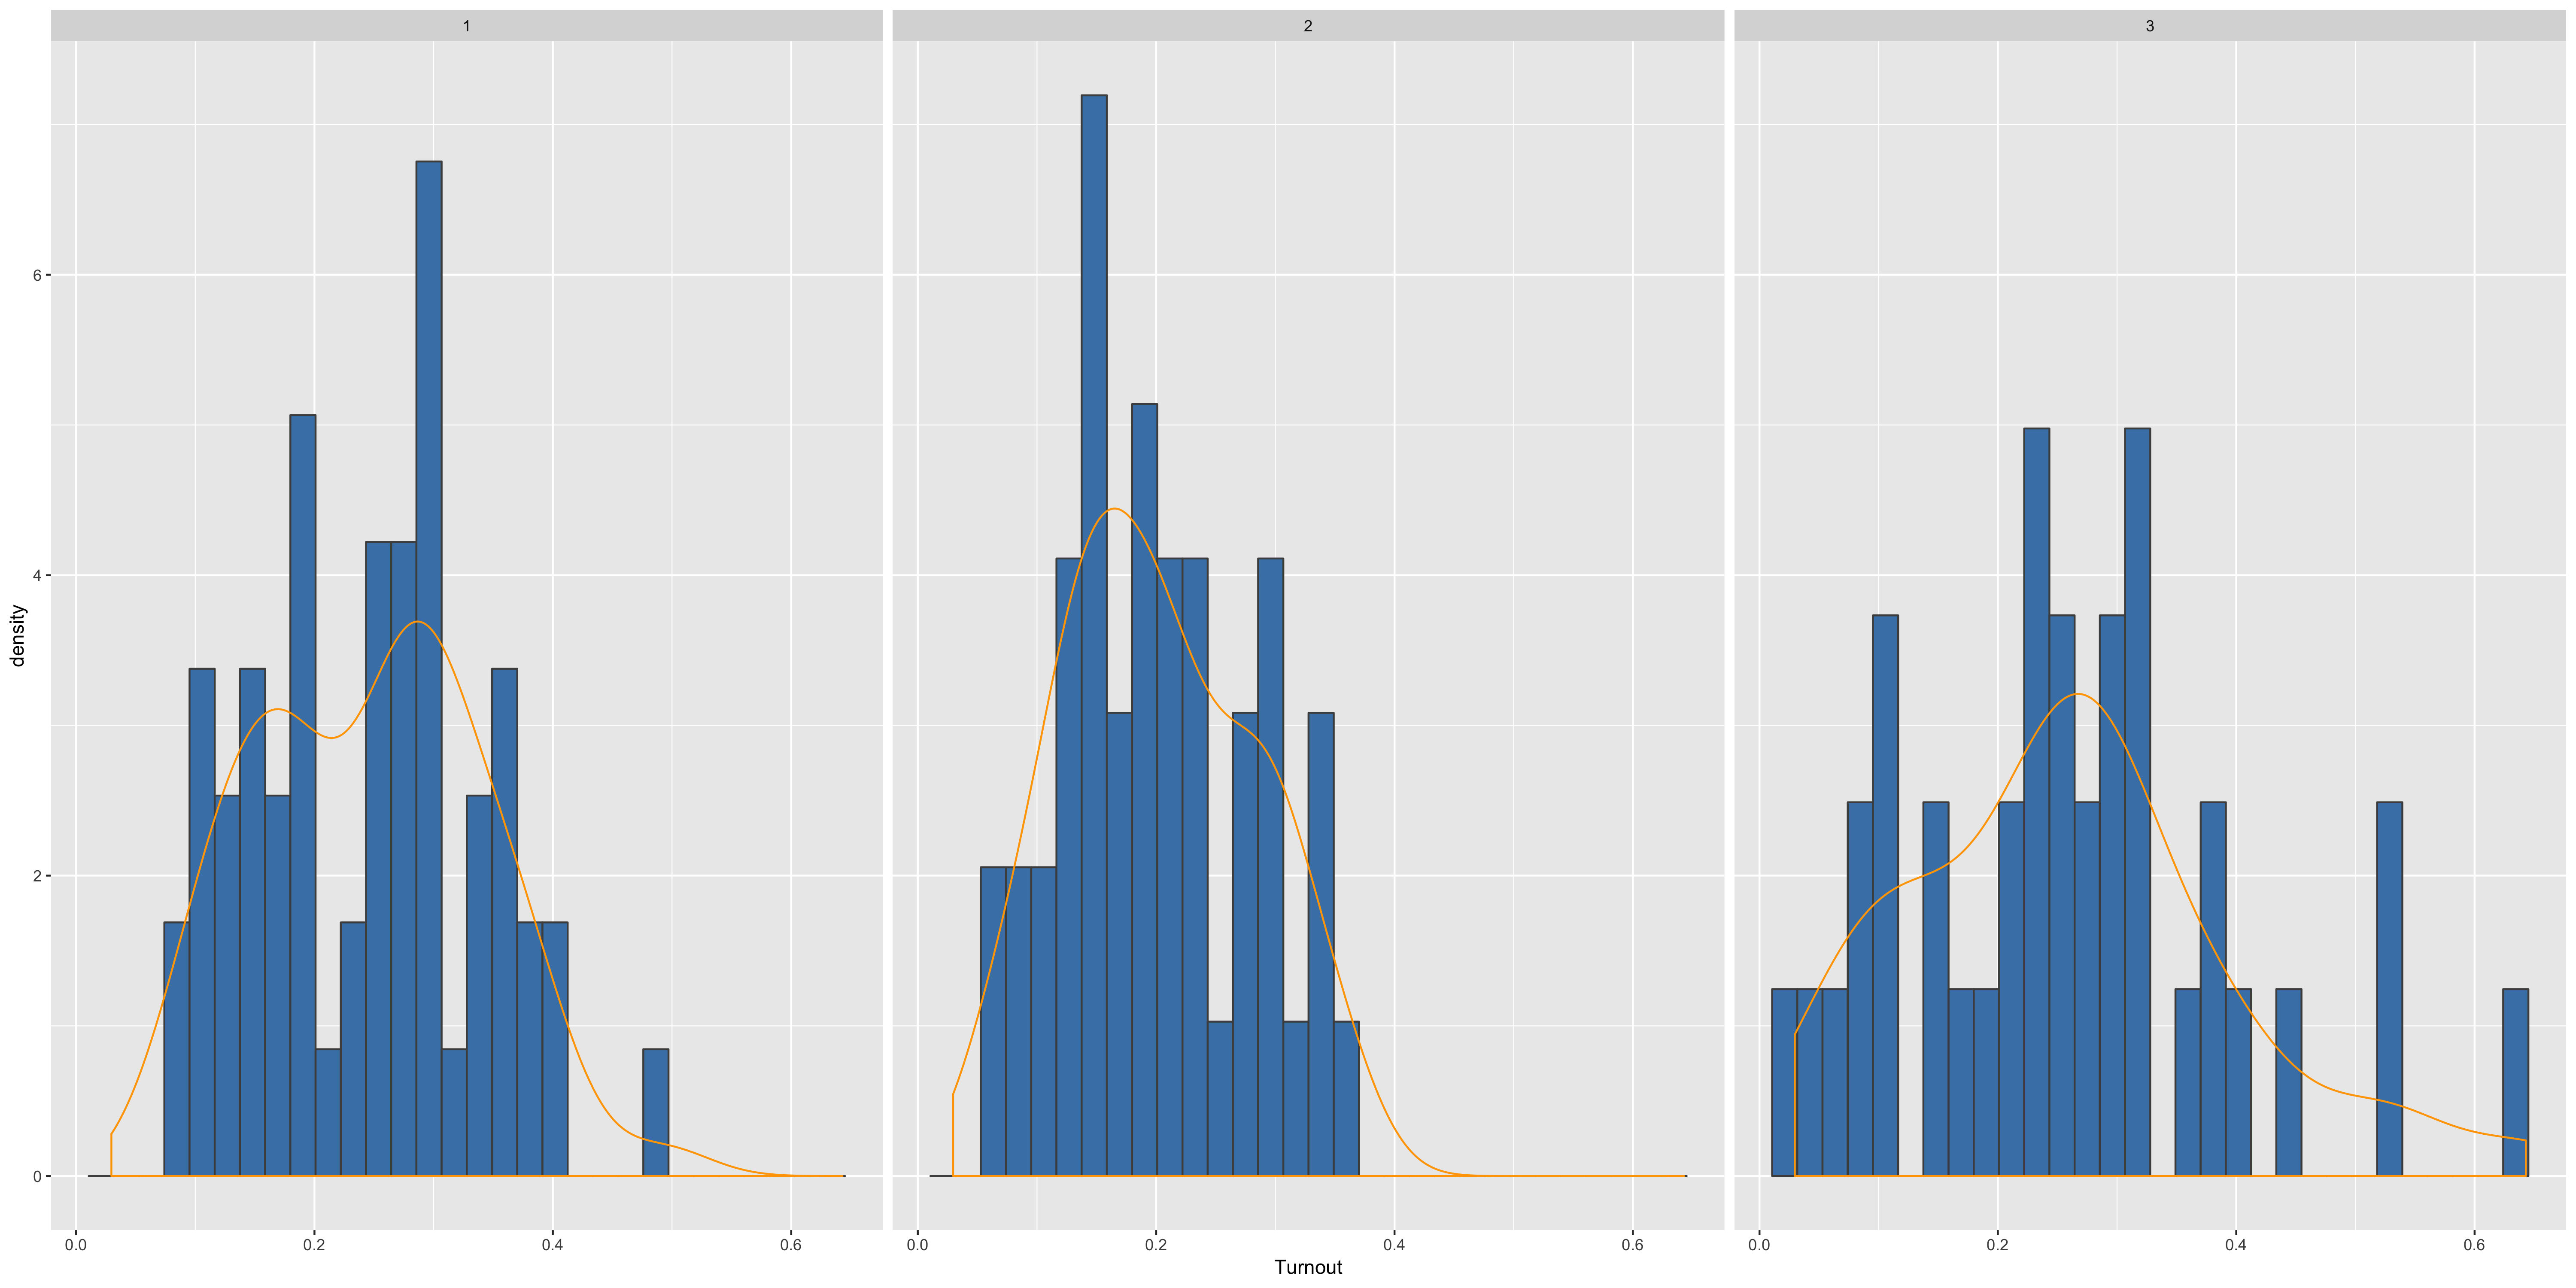
\includegraphics[width=0.4\textwidth, center]{hs}
		\caption{Histogram of Primary Turnout by Type}
		\label{fig:figure2}
	\end{figure}
	\textit{Figure 3} shows a scatterplot of turnout by type. The average turnout of open primaries appear to be higher than that of closed primaries. Mixed primaries appear far more variant than its counterparts. 
		\begin{figure}[H]
			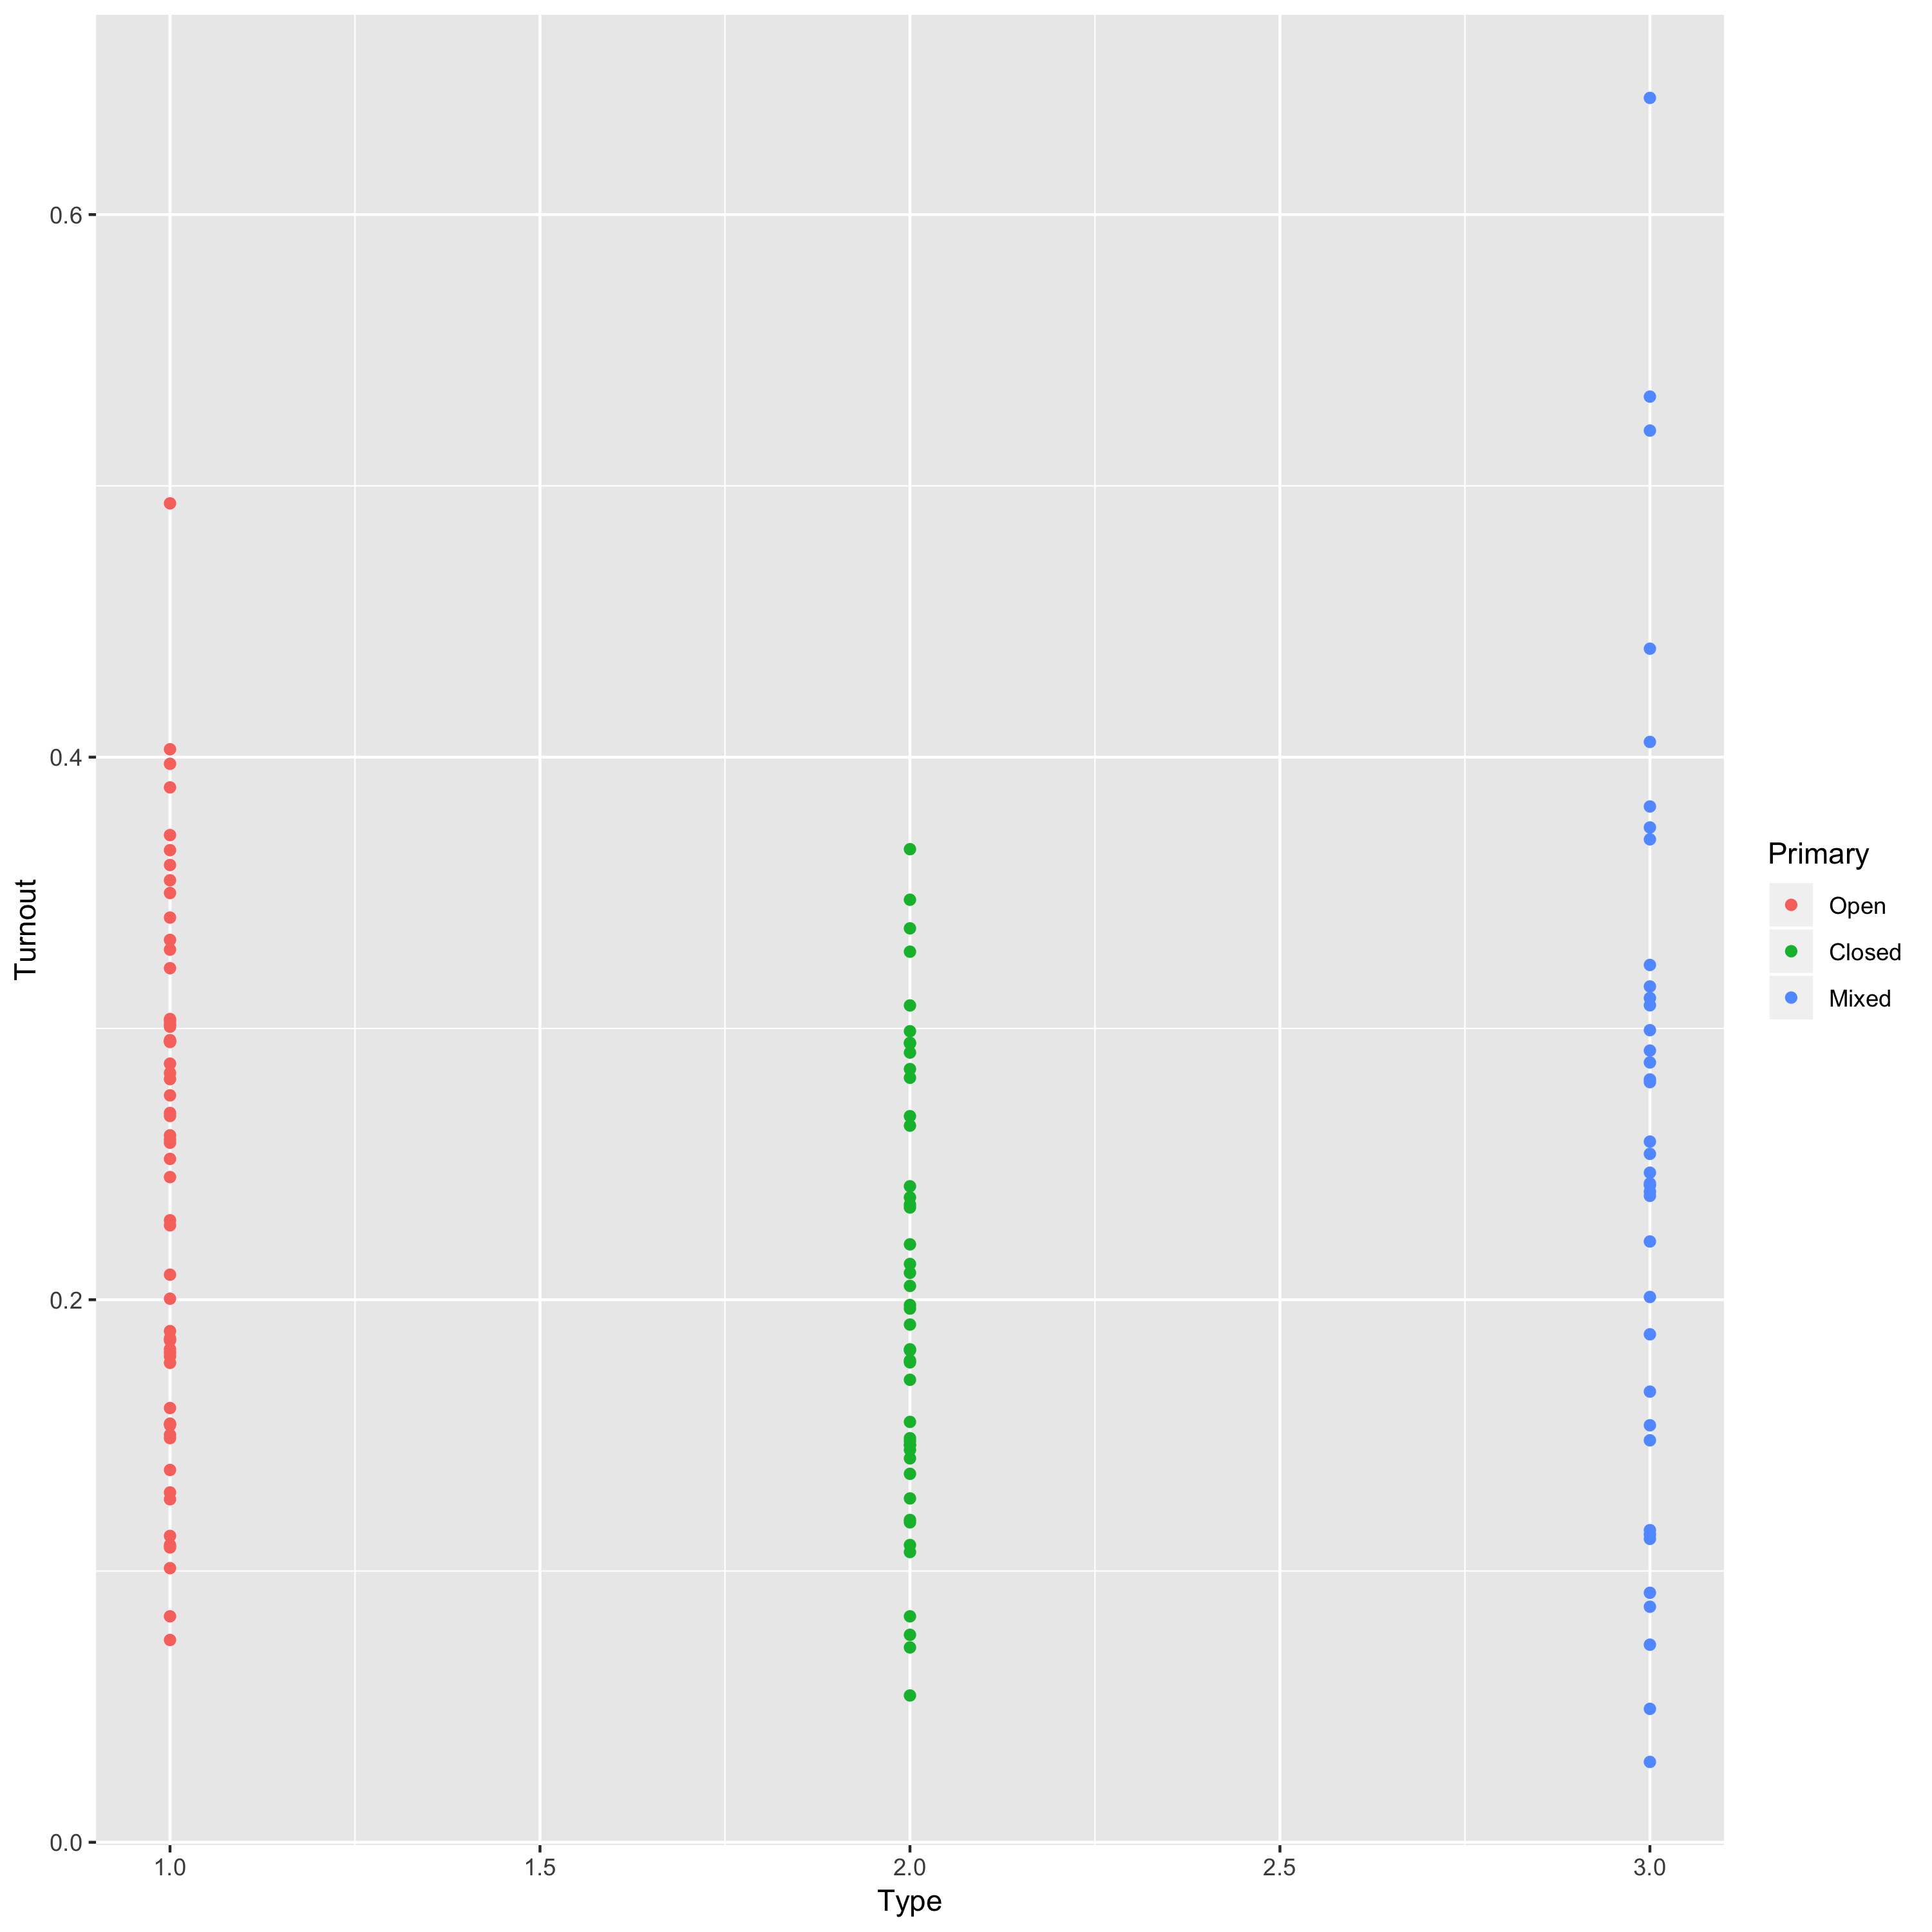
\includegraphics[width=0.4\textwidth, center]{scatter}
			\caption{Scatterplot of Turnout by Type}
			\label{fig:figure3}
		\end{figure}
	\textit{Table 2} displays turnout summary statistics by type and affirms these visual trends. Open primaries and mixed primaries have higher turnout than closed primaries, and mixed primaries have a higher standard deviation. \par
	\textit{Table 3} shows the turnout summary statistics broken up by year. Both incumbent years 2004 and 2012 had lower average turnout. 2000, a non-incumbent year, also had low turnout, comparable to the incumbent years. This may be fueled by Al Gore's Democratic candidacy, which failed to see a serious challenger, particularly in later elections.
		\end{doublespace}
		\begin{table}[H]
			\begin{center}
				\begin{scriptsize} 
					\caption{Turnout Summary Statistics}
					\begin{tabular} {l r r r r r r r r }
						\multicolumn{ 8 }{l}{  } \cr 
						\hline Variable  &   {vars} &  {n} &  {mean} &  {sd} &  {min} &  {max} &  {range} &  {se}\cr 
						\hline 
						Turnout   &  1  &  140  &  0.23  &  0.11  &  0.03  &  0.64  &  0.61  &  0.01 \cr 
						\hline 
					\end{tabular}
					\vspace{1em}
					\caption{Turnout Summary Statistics by Type}
					\begin{tabular} {l r r r r r r r r }
						\multicolumn{ 8 }{l}{  } \cr 
						\hline Variable  &   {vars} &  {n} &  {mean} &  {sd} &  {min} &  {max} &  {range} &  {se}\cr 
						\hline 
						Open   &  1  &  56  &  0.25  &  0.10  &  0.07  &  0.49  &  0.42  &  0.01 \cr 
						Closed   &  1  &  46  &  0.20  &  0.08  &  0.05  &  0.37  &  0.31  &  0.01 \cr 
						Mixed   &  1  &  38  &  0.26  &  0.14  &  0.03  &  0.64  &  0.61  &  0.02 \cr 
						\hline 
					\end{tabular}
					\vspace{1em}
					\caption{Turnout Summary Statistics by Year}
					\begin{tabular} {l r r r r r r r r }
						\multicolumn{ 8 }{l}{  } \cr 
						\hline Variable  &   {vars} &  {n} &  {mean} &  {sd} &  {min} &  {max} &  {range} &  {se}\cr 
						\hline 
						2000   &  1  &  33  &  0.18  &  0.09  &  0.05  &  0.44  &  0.39  &  0.01 \cr 
						2004   &  1  &  21  &  0.17  &  0.08  &  0.05  &  0.30  &  0.25  &  0.02 \cr 
						2008   &  1  &  34  &  0.30  &  0.07  &  0.18  &  0.53  &  0.36  &  0.01 \cr 
						2012   &  1  &  23  &  0.19  &  0.12  &  0.03  &  0.64  &  0.61  &  0.02 \cr 
						2016   &  1  &  29  &  0.31  &  0.08  &  0.18  &  0.52  &  0.34  &  0.02 \cr 
						\hline 
					\end{tabular}
				\end{scriptsize}
			\end{center}
			\label{default}
		\end{table} 
	\begin{doublespace}
	\subsection*{t-Tests}
	Three comparison of mean t-Tests will be run in Stata. The tests compare open primaries and mixed primaries, closed primaries and mixed primaries, and open primaries and closed primaries. The tests will compare the null hypotheses that that the mean turnouts are equal to three alternatives: that type has higher average turnout than type b, that type a and type b have different average turnouts, and that type a has lower average turnout than type b. 
	\subsection*{Regressions}
	For regressions will be run in R. Each model will regress \textit{Turnout} on \textit{Type} and yearly fixed effects dummies. 
	Model 1 will not add any extra control variables:
	\begin{center}
		$Turnout = \beta_{0} + \beta_{1}Type_{it} + \delta_{1}2000_{i} + \delta_{2}2004_{i} + \delta_{3}2008_{i} + \delta_{4}2012_{i} + \delta_{5}2016_{i}$\par
	\end{center}
	Model 2 will include control variables for \textit{Month} the number of months between the election and party conventions. While each party's conventions were not held in the same month every year, they were usually within a week of each other and at least a month from the last primary – the shorter time period was chosen in these instances. For the very small number of states (less than 5) where primaries were not held in the same month, the shorter time period was also chosen. Model 2 will also include \textit{White} the percent of a state's population that was white and \textit{Unemp} the state's unemployment rate. \par
	\begin{center}
		$Turnout = \beta_{0} + \beta_{1}Type_{it} + \beta_{2}Month_{it} + \beta_{3}White_{it} + \beta_{4}Unemp_{it} + \delta_{1}2000_{i} + \delta_{2}2004_{i} + \delta_{3}2008_{i} + \delta_{4}2012_{i} + \delta_{5}2016_{i}$\par
	\end{center}
	Model 3 will drop the \textit{White} variable from Model 2 but will keep \textit{Month} and \textit{Unemp}. \par
	\begin{center}
		$Turnout = \beta_{0} + \beta_{1}Type_{it} + \beta_{2}Month_{it} + \beta_{3}Unemp_{it} + \delta_{1}2000_{i} + \delta_{2}2004_{i} + \delta_{3}2008_{i} + \delta_{4}2012_{i} + \delta_{5}2016_{i}$ \par
	\end{center}
	Model 4 will drop \textit{Month} from Model three but will keep \textit{Unemp}.
	\begin{center}
		$Turnout = \beta_{0} + \beta_{1}Type_{it} + \beta_{2}Unemp_{it} + \delta_{1}2000_{i} + \delta_{2}2004_{i} + \delta_{3}2008_{i} + \delta_{4}2012_{i} + \delta_{5}2016_{i}$
	\end{center}
	\section{Results}
	\subsection*{t-Tests}
	The first t-test compared open primaries (1) and closed primaries (3), seen in \textit{Figure 3}. Across the three alternate hypotheses (that open primaries had lower turnout than mixed primaries, that open and mixed primaries had different turnout, and that open primaries had higher turnout than mixed primaries), none were significant. This finding goes against the theory that open primaries will have more turnout than mixed primaries. The votes of dissenting counter-partisans, the only difference between open and mixed primaries, do not appear to have a significant impact on turnout rates. \par
	\begin{figure}[h]
		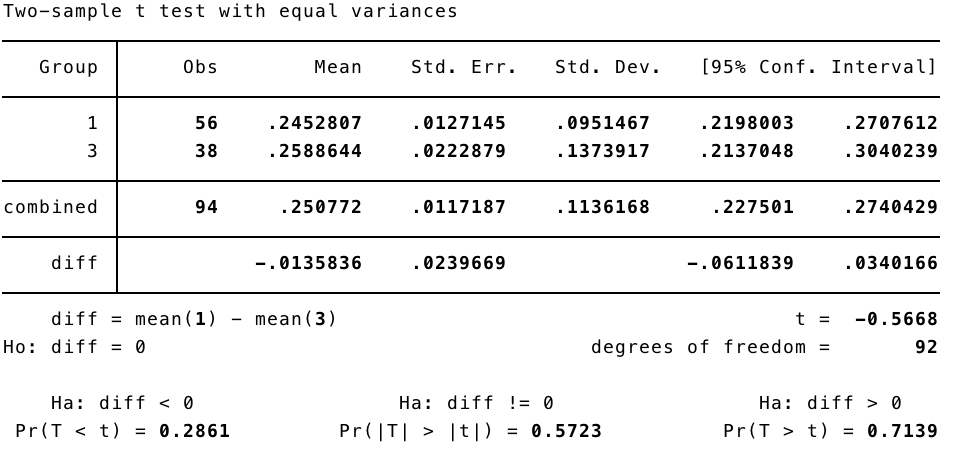
\includegraphics[width=0.5\textwidth, center]{1}
		\caption{Comparison of Means t-Test of Open and Mixed Primaries}
		\label{fig:figure4}
	\end{figure}
	\begin{figure}[h]
		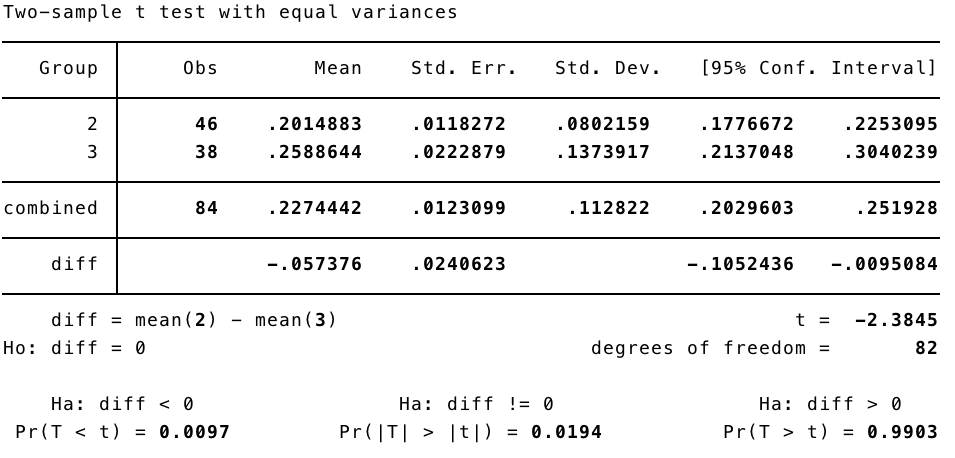
\includegraphics[width=0.5\textwidth, center]{2}
		\caption{Comparison of Means t-Test of Closed and Mixed Primaries}
		\label{fig:figure5}
	\end{figure}
	\begin{figure}[H]
		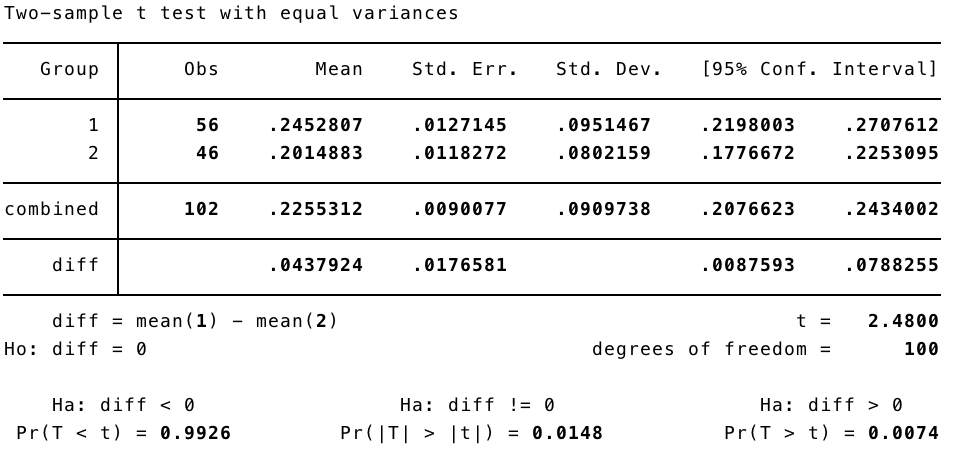
\includegraphics[width=0.5\textwidth, center]{3}
		\caption{Comparison of Means t-Test of Open and Closed Primaries}
		\label{fig:figure6}
	\end{figure}
	In the second t-test of closed (2) to mixed primary turnout, seen in \textit{Figure 4}, the hypothesis that closed primary turnout is less than mixed primary turnout was significant at the 0.01 level, allowing the rejection of the null hypothesis that the mean turnouts are the same. \par
	In the final t-test, between open primaries to closed primaries, seen in \textit{Figure 5}, the alternate hypothesis that open primaries have greater turnout than closed primaries was significant at the 0.01 level, allowing the rejection of the null hypothesis that the mean turnouts are the same. \par
	Overall, these support the hypothesis that closed primary turnout is lower than open and mixed primary turnout. Despite this significance, the relationship between turnout and primary type may be fueled by exogenous factors not accounted for in a comparison of means t-test. This also demonstrates the importance of independent voters in determining turnout. Open and mixed primary turnouts were not significantly different, but both were significantly higher than closed turnout. Independents, who make up a plurality of the population (Jones 2018),  have an impact on turnout rates causing both open and mixed primaries to have higher levels of turnout. Dissenting counter-partisans, on the other hand, have little effect as evident by the lack of a significant difference between open and mixed turnouts. \par
	\begin{figure}[h]
		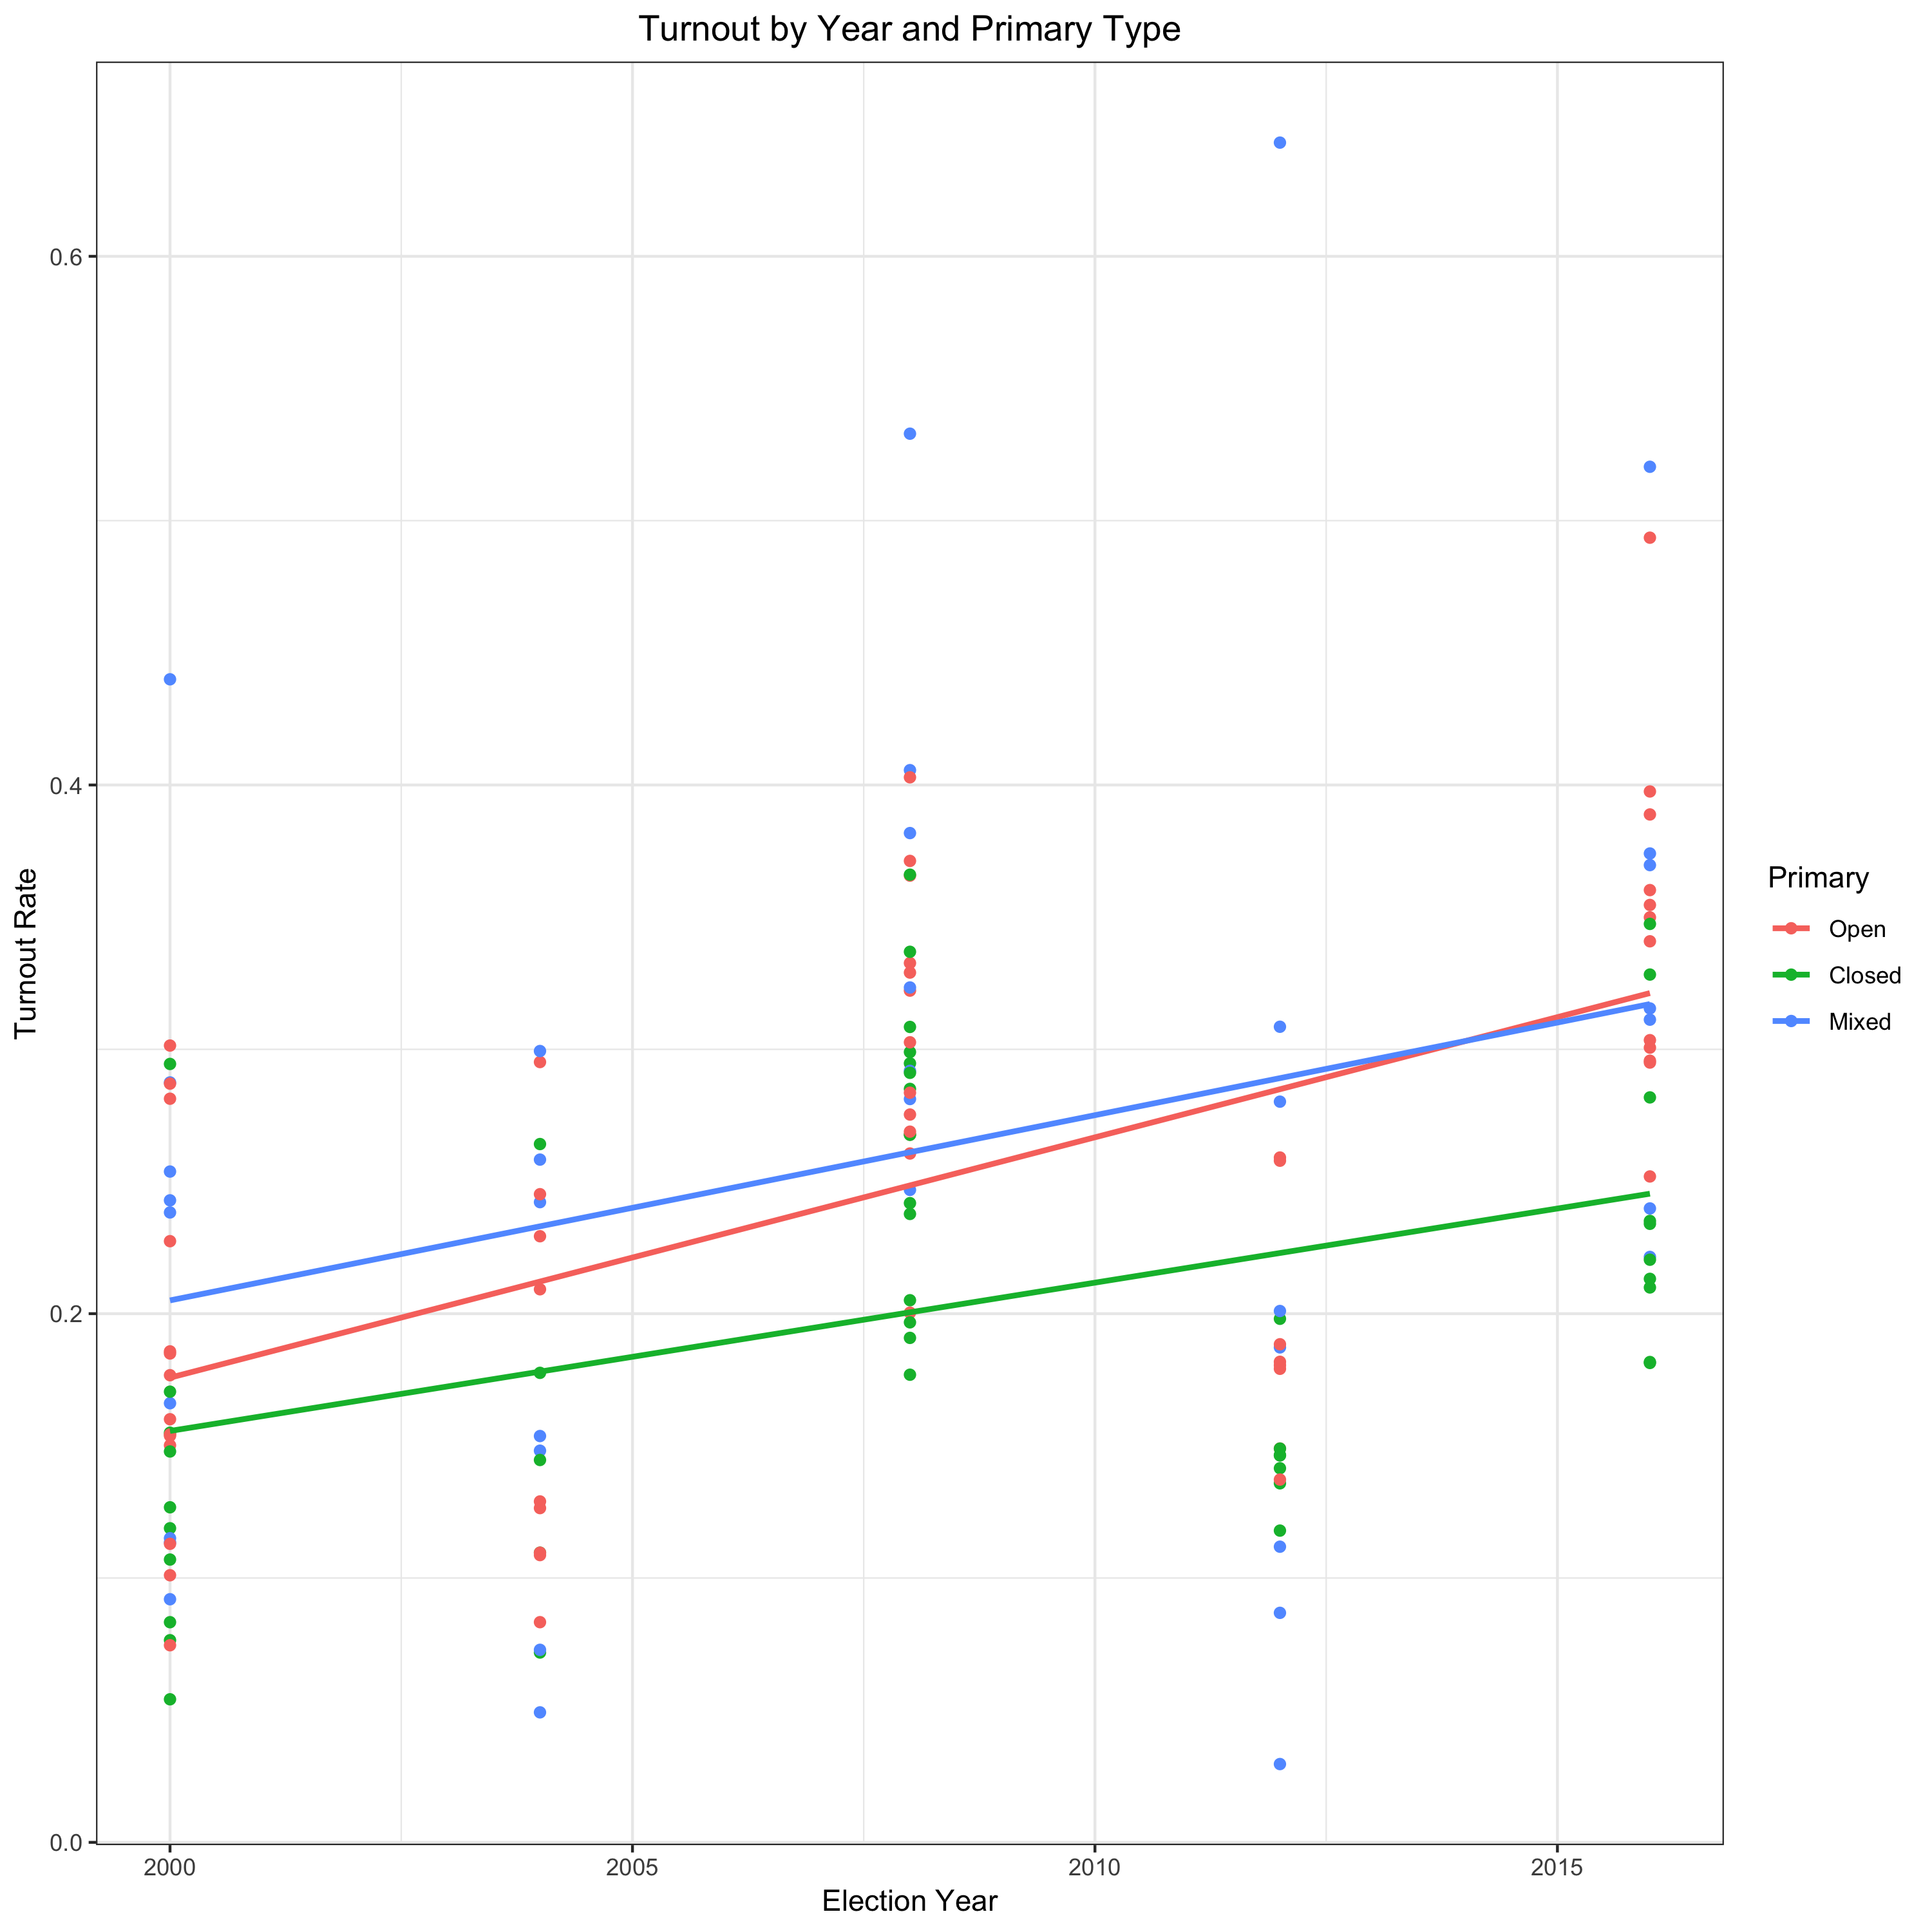
\includegraphics[width=0.5\textwidth, center]{line}
		\caption{Turnout over Time by Type}
		\label{fig:figure7}
	\end{figure}
	When turnout is plotted against year and fit curves are drawn for each primary type, as in \textit{Figure 7}, the difference in turnout between type and year and be visualized. While turnout for all primary types increases over time, the curve for closed primaries is notably lower than the curves for the closed and mixed primaries. Interestingly, until 2016, mixed primaries had higher average turnout than open primaries. Also, the average turnout values for non-incumbent years appears to be higher for all primary types, possibly contributing to the positive trends, as the most recent election was a non-incumbent election.
	\subsection*{Regressions}
	\textit{Table 4} displays the coefficient estimates for the four models. In none of the four regressions was \textit{Type} significant. This strongly refutes the hypothesis that primary rules explain primary turnout. In model one, all of the year dummies were significant and positive. In model three, the time dummies and the variable \textit{Unemp} were significant. The year dummies remained positive; the unemployment variable was negative with a magnitude of 0.015, so that for every one percentage point increase in a state's unemployment, primary turnout would decrease by 0.015 percentage points. \par
	Model four dropped the insignificant \textit{Month} variable. \textit{Unemp} remained significant and around the same value as in model three. \par
	Model two was by far the most interesting model, where the variable \textit{White} picked up both a practically and statistically significant coefficient. For every percentage point increase in the proportion of a state that is white, turnout increases by 0.283 percentage points. A state's racial composition has a significant impact on primary turnout, taking away significance from all other variables, time dummies included.\par
	In all four models, incumbent years had a smaller effect than non-incumbent years. In model two, the incumbent year estimates were negative, suggesting that incumbent years not only had a smaller effect on turnout but actively decreased it; however, the coefficients were insignificant. This provides some credence to the theory that incumbent primaries generally see lower turnout.\par
	It is also worth noting that each of these models has an adjusted R$^{2}$ value above 0.885, meaning that the models explain at least 88.5\% of the variation in the data. This high R$^{2}$ value indicates that each of the models is a relatively good fit for the data.
\end{doublespace}
		\begin{table}[H] \centering 
		\caption{Regressions of Turnout on Type} 
		\label{} 
		\small 
		\begin{tabular}{@{\extracolsep{5pt}}lcccc} 
			\\[-1.8ex]\hline 
			\hline \\[-1.8ex] 
			& \multicolumn{4}{c}{\textit{Dependent variable:}} \\ 
			\cline{2-5} 
			\\[-1.8ex] & \multicolumn{4}{c}{Turnout} \\ 
			\\[-1.8ex] & (1) & (2) & (3) & (4)\\ 
			\hline \\[-1.8ex] 
			Type & 0.007 & 0.002 & 0.005 & 0.005 \\ 
			& (0.009) & (0.009) & (0.009) & (0.009) \\ 
			& & & & \\ 
			Month &  & 0.005 & 0.003 &  \\ 
			&  & (0.006) & (0.006) &  \\ 
			& & & & \\ 
			White &  & 0.283$^{***}$ &  &  \\ 
			&  & (0.064) &  &  \\ 
			& & & & \\ 
			Unemp &  & $-$0.003 & $-$0.015$^{**}$ & $-$0.016$^{**}$ \\ 
			&  & (0.007) & (0.007) & (0.007) \\ 
			& & & & \\ 
			2000 & 0.164$^{***}$ & $-$0.070 & 0.217$^{***}$ & 0.232$^{***}$ \\ 
			& (0.023) & (0.079) & (0.049) & (0.036) \\ 
			& & & & \\ 
			2004 & 0.154$^{***}$ & $-$0.077 & 0.232$^{***}$ & 0.245$^{***}$ \\ 
			& (0.026) & (0.086) & (0.055) & (0.046) \\ 
			& & & & \\ 
			2008 & 0.285$^{***}$ & 0.060 & 0.360$^{***}$ & 0.380$^{***}$ \\ 
			& (0.022) & (0.089) & (0.062) & (0.046) \\ 
			& & & & \\ 
			2012 & 0.178$^{***}$ & $-$0.029 & 0.289$^{***}$ & 0.306$^{***}$ \\ 
			& (0.026) & (0.097) & (0.071) & (0.060) \\ 
			& & & & \\ 
			2016 & 0.294$^{***}$ & 0.107 & 0.365$^{***}$ & 0.378$^{***}$ \\ 
			& (0.023) & (0.075) & (0.051) & (0.042) \\ 
			& & & & \\ 
			\hline \\[-1.8ex] 
			Observations & 140 & 140 & 140 & 140 \\ 
			R$^{2}$ & 0.890 & 0.908 & 0.894 & 0.894 \\ 
			Adjusted R$^{2}$ & 0.885 & 0.902 & 0.888 & 0.889 \\ 
			Residual Std. Error & 0.087 (df = 134) & 0.081 (df = 131) & 0.086 (df = 132) & 0.086 (df = 133) \\ 
			\hline 
			\hline \\[-1.8ex] 
			\textit{Note:}  & \multicolumn{4}{r}{$^{*}$p$<$0.1; $^{**}$p$<$0.05; $^{***}$p$<$0.01} \\ 
		\end{tabular} 
	\end{table} 
\begin{doublespace}
		When models were compared in a series of two-regression ANOVA tests, shown in \textit{Appendix I}, model two appeared to be a significantly better fit for the data than any of the other models. \par
		The relationship between primary rules and turnout appears to be one of little causal significance, despite the significant differences in means.
		
		\section{Discussion} 
		The findings of this research fit in neatly with the general uncertainty about primary rules’ effects on turnout. Despite significant differences in the averages turnout between open and mixed versus closed primaries, none of the regressions showed a significant coefficient on the primary rules’ variable. The lack of a significant difference in the mean turnout of open and mixed primaries indicates that independent voters do not have a significant impact on turnout. Gallup polling shows that independents make up a plurality of the population (Jones 2018). Despite Jones' results, some have argued independents are less politically engaged than partisan voters (Hillygus \&
Shields 2008; Keith et al. 1992). These findings contrast that arugument, showing that independent voters do turnout signficantly. Because of the effect of independent voters, mixed primaries may be ideal for state parties who wish to maintain the integrity of their primary by not allowing in counter-partisans while still being able to see increased turnout. Many independents ``lean" to one side of the aisle or another and act similarly to weak partisans (Magleby, Nelson, \& Westlye 2011; Klar 2014). This tendency for independents to lean may make them more inclined to vote for their marginally preferred party if given the opportunity. It appears from these findings that counter-partisans are not apt to vote for the other side, a trend possibly exacerbated by increased hostility between parties (Lelkes 2016; cf. Kauffman, Gimpel, \& Hoffman 2003).  \par
		Another key finding was the significant impact of race on primary turnout. In the regression that included the percent of the population that was white in a state, none of the other explanatory variables' coefficients were significant. This finding plays into a broader narrative that whites are significantly more likely to vote than racial minorities. Research suggests that minority voters do not turnout for a number of reasons. For one, Black and Latino voters in particular are subject to socioeconomic degeneration: less educated, lower income individuals are less likely to vote (Tate 1991; Highton \& Wolfinger 2001; Xu 2005). There is also evidence that recent immigration and length of residency of minorities, particularly Asian and Latin Americans, is correlated to turnout: more recent immigrants are less likely to vote (Xu 2005). Perhaps more pertinently, Kauffman, Gimpel, \& Hoffman (2003) suggest that more homogenous localities see higher turnout. States that are more homogenous and, therefore, have a higher proportion of white citizens, are more likely to turnout as model two suggests. \par
		The variable measuring the period of time between the a primary and the parties’ conventions in months lacked significance in all three of the models in which it was used. This contrasts the idea that front-loading in the primary cycle has a significant impact on low voter turnout, particularly in later elections (Steger 2007; Mayer \& Busch 2004; Fredrick 2012; McDonald \& Merivaki 2015; cf. Jewitt 2014). \par
		Incumbent elections appear to have depressed turnout in these models. This depression may be explained by voters losing motivation in the incumbent’s party. When an incumbent fails to see a serious challenge and primaries are cancelled, a message is sent to the voter that their votes do not matter, and the incumbent will be nominated either way. McDonald \& Merivaki’s (2015) findings support this conclusion. \par
		There are some important limitations of this study. While many previous studies of primary turnout have relied upon individual likelihood probit or logit regressions (e.g. Oliver 1996; Xu 2005; Hersh \& Ghitza 2018), this model relies on a linear fixed-effects model of aggregate VEP turnout data. This form of regression limits what variables we can test. In particular, individual level variables that may impact turnout are not able to be properly accounted for. The method of measuring primary type as a categorical variable may have been problematic. In future research, the categorical variable should be measured as an ordinal variable, tracking ``openness” linearly, so that mixed primaries take a value in between the values of open and closed primaries. As it stands, the current variable cannot properly measure the effects of changes in rule openness as it jumps from more open to less open and back to more open between the values of one, two, and three. This possibly led to the failure of the models to produce a significant output for primary type. Combining both parties in a state may have caused the model to lose a bit of nuance, or at the very least, causes a notable drop in the number of potential data points. Despite these limitations, this paper fills an important niche in the literature, examining the effect of primary type on turnout without using dummy variables and across parties. The model also reveals important findings on the relationship between race and primary turnout and about the role of incumbent elections on turnout.    
		\section*{Bibliography}
		\begin{hangparas}{.25in}{1}
			Frederick, Heather. 2012. “Reforming the Presidential Primary System: The Voter Turnout Initiative.” \textit{PS: Political Science and Politics} 45(1): 51-57.
			
			Gans, Curtis. 2010. “Final Primary Report: 2010 Elections.” \textit{Center for the Study of the American Electorate}. 
			
			Geer, John G. 1986. “Rules Governing Presidential Primaries.” \textit{The Journal of Politics} 48(4): 1006-1025.
			
			Gerber, Alan S., Gregory A. Huber, Daniel R. Biggers, and David J. Hendry. 2017. “Why Don’t People Vote in U.S. Primary Elections? Assessing Theoretical Explanations for Reduced Participation.” \textit{Electoral Studies} 45(1): 119-129.
			
			Hersh, Eitan, and Yair Ghitza. 2018. “Mixed Partisan Households and Electoral Participation in the United States.” \textit{PLoS One} 13(10): e0203997.
			
			Highton, Benjamin, and Raymond E. Wolfinger. 2001. “The First Seven Years of the Political Life Cycle.”\textit{ American Journal of Political Science} 45(1): 202-209.
			
			Hillygus, D. Sunshine, and Todd G. Shields. 2009. \textit{The Persuadable Voter: Wedge Issues in Presidential Campaigns}. Princeton, NJ: Princeton University Press. 
			
			Jewitt, Caitlin E. 2014. “Packed Primaries and Empty Caucuses: Voter Turnout in Presidential Nominations.” \textit{Public Choice} 160(1): 295-312.
			
			Jones, Jeffrey M. 2018. “Americans' Identification as Independents Back Up in 2017.” \textit{Gallup}, January 8. https://news.gallup.com/poll/225056/americans-identification-independents-back-2017.aspx
			
			Kaufmann, Karen M., James G. Gimpel, and Adam H. Hoffman. 2003. “A Promised Fulfilled? Open Primaries and Representation.” \textit{The Journal of Politics} 65(2): 457-476.
			
			Keith, Bruce E., David B. Magleby, Candice J. Nelson, Elizabeth A. Orr, Mark C. Westlye, and Raymond E. Wolfinger. 1992. \textit{The Myth of the Independent Voter}. Oakland, CA: University of California Press.
			
			Klar, Samara. 2014. ``Identity and Engagement among Political Independents in America." \textit{International Society of Political Psychology} 35(4): 577-591.
			
			Lelkes, Yphtach. 2016. ``Mass Polarization: Manifestations and Measurements." \textit{Public Opinion Quarterly} 80(Special Issue): 392-410
		
			Magleby, David B., Candice J. Nelson, and Mark C. Westlye. 2011. ``The Myth of the Independent Voter Revisited." In \textit{Facing the Challenge of Democracy: Explorations in the Analysis of Public Opinion and Political Participation}, eds. Paul M. Sniderman and Benjamin Highton, 238-264. Princeton, NJ: Princeton University Press
		
			Mayer, William G., and Andrew E. Busch. 2004. \textit{The Front-Loading Problem in Presidential Nominations}. Washington, D.C.: Brookings Institution Press. 	
		
			McDonald, Michael P., and Thessalia Merivaki. 2015. “Voter Turnout in Presidential Nominating Contests.” The Forum 13(4): 597-622.
			
			Norrander, Barbara, and Gregg W. Smith. 1985. “Type of Contest, Candidate Strategy, and Turnout in Presidential Primaries.” \textit{American Politics Quarterly} 13(1): 28-50.
			
			Oliver, J. Eric. 1996. “The Effects of Eligibility Restrictions and Party Activity on Absentee Voting and Overall Turnout.” \textit{American Journal of Political Science} 40(2): 498-513. 
		
			Patterson, Thomas E. 2009. 	“Voter Participation: Records Galore This Time, but What about Next Time?” In \textit{Reforming the Presidential Nomination Process}, eds. Steven S. Smith and Melanie J. Springer, 44-63. Washington, D.C.: Brookings Institution Press. 
		
			Ranney, Austin. 1977. \textit{Participation in American Presidential Nominations, 1976}. Washington, D.C.: American Enterprise Institute for Public Policy Research. 
			
			Steger, Wayne P. 2007. “Who Wins Nominations and Why?” \textit{Political Research Quarterly} 60(1): 91-99. 
		
			Tate, Katherine. 1991. “Black Political Participation in the 1984 and 1988 Presidential Elections.” \textit{The American Political Science Review} 85(4): 1159-1176. 
			
			Xu, Jun. 2005. “Why Do Minorities Participate Less? The Effects of Immigration, Education, and Electoral Process on Asian American Voter Registration and Turnout.” \textit{Social Science Research} 34(4): 682-702.
		\end{hangparas}
\end{doublespace}



		









\section*{Appendix I: ANOVA Tests}
\begin{doublespace}
	The ANOVA tests can be read as a comparison between more and less complex models. Models increase in complexity in the order of 1, 4, 3, and 2. When the ANOVA test is run between two models, the null hypothesis is that the simpler model is a better fit. If the more complex model has a significant F-statistic, then the null hypothesis is rejected, and the more complex model is a better fit. In \textit{Table 5}, the null hypothesis is rejected and  model four is deemed a better fit than model one. In \textit{Table 6}, models three and four were compared, and model three, the more complex model, failed to have a significant F-statistic, meaning that the null hypothesis failed to be rejected and model four was a better model. In \textit{Tables 7 \& 8}, model two, the most complex model, is compared to models four and one, respectively. In both instances, the null hypothesis was rejected and model two was considered a better fit for the data, meaning that model two was the best fit overall.
	
\end{doublespace}
 
	
	
	\begin{table}[H]
	\centering
	\vspace{2em}
	\caption{ANOVA of Models 1 and 4}
	\begin{tabular}{lrrrrrr}
		\hline
		& Res.Df & RSS & Df & Sum of Sq & F & Pr($>$F) \\ 
		\hline
		1 & 134 & 1.02 &  &  &  &  \\ 
		4 & 133 & 0.98 & 1 & 0.04 & 5.59 & 0.0195* \\ 
		\hline
		\hline \\[-1.8ex] 
		\textit{Note:}  & \multicolumn{4}{r}{$^{*}$p$<$0.1; $^{**}$p$<$0.05; $^{***}$p$<$0.01} \\
	\end{tabular}
	\vspace{2em}
	\caption{ANOVA of Models 4 and 3}
	\begin{tabular}{lrrrrrr}
		\hline
		& Res.Df & RSS & Df & Sum of Sq & F & Pr($>$F) \\ 
		\hline
		4 & 133 & 0.98 &  &  &  &  \\ 
		3 & 132 & 0.98 & 1 & 0.00 & 0.20 & 0.6518 \\ 
		\hline
		\hline \\[-1.8ex] 
		\textit{Note:}  & \multicolumn{4}{r}{$^{*}$p$<$0.1; $^{**}$p$<$0.05; $^{***}$p$<$0.01} \\
	\end{tabular}
	\vspace{2em}
	\caption{ANOVA of Models 4 and 2} 
	\begin{tabular}{lrrrrrr}
		\hline
		& Res.Df & RSS & Df & Sum of Sq & F & Pr($>$F) \\ 
		\hline
		4 & 133 & 0.98 &  &  &  &  \\ 
		2 & 131 & 0.85 & 2 & 0.13 & 10.06 & 0.0001*** \\ 
		\hline
		\hline \\[-1.8ex] 
		\textit{Note:}  & \multicolumn{4}{r}{$^{*}$p$<$0.1; $^{**}$p$<$0.05; $^{***}$p$<$0.01} \\
	\end{tabular}
	
	\vspace{2em}
	\caption{ANOVA of Models 1 and 2}
	\begin{tabular}{lrrrrrr}
		\hline
		& Res.Df & RSS & Df & Sum of Sq & F & Pr($>$F) \\ 
		\hline
		1 & 134 & 1.02 &  &  &  &  \\ 
		2 & 131 & 0.85 & 3 & 0.17 & 8.82 & 0.0000*** \\ 
		\hline
		\hline \\[-1.8ex] 
		\textit{Note:}  & \multicolumn{4}{r}{$^{*}$p$<$0.1; $^{**}$p$<$0.05; $^{***}$p$<$0.01} \\
	\end{tabular}
	
\end{table}

\section*{Appendix II: Code}
\subsection*{R}
\lstinputlisting{DSP.R}
\subsection*{Stata}
\lstinputlisting{DSP.do}
\end{document}